\documentclass[12pt]{article}
\setlength\parindent{0pt}
\usepackage{fullpage}
\usepackage[margin=0.5in]{geometry}
\usepackage{amsmath}
\usepackage{pdflscape}
\usepackage{color}
\usepackage{graphicx}
\setlength{\parskip}{4mm}
\def\LL{\left\langle}   % left angle bracket
\def\RR{\right\rangle}  % right angle bracket
\def\LP{\left(}         % left parenthesis
\def\RP{\right)}        % right parenthesis
\def\LB{\left\{}        % left curly bracket
\def\RB{\right\}}       % right curly bracket
\def\PAR#1#2{ {{\partial #1}\over{\partial #2}} }
\def\PARTWO#1#2{ {{\partial^2 #1}\over{\partial #2}^2} }
\def\PARTWOMIX#1#2#3{ {{\partial^2 #1}\over{\partial #2 \partial #3}} }
\newcommand{\BE}{\begin{displaymath}}
\newcommand{\EE}{\end{displaymath}}
\newcommand{\BNE}{\begin{equation}}
\newcommand{\ENE}{\end{equation}}
\newcommand{\BEA}{\begin{eqnarray}}
\newcommand{\EEA}{\nonumber\end{eqnarray}}
\newcommand{\EL}{\nonumber\\}
\newcommand{\la}[1]{\label{#1}}
\newcommand{\ie}{{\em i.e.\ }}
\newcommand{\eg}{{\em e.\,g.\ }}
\newcommand{\cf}{cf.\ }
\newcommand{\etc}{etc.\ }
\newcommand{\Tr}{{\rm tr}}
\newcommand{\etal}{{\it et al.}}
\newcommand{\OL}[1]{\overline{#1}\ } % overline
\newcommand{\OLL}[1]{\overline{\overline{#1}}\ } % double overline
\newcommand{\OON}{\frac{1}{N}} % "one over N"
\newcommand{\OOX}[1]{\frac{1}{#1}} % "one over X"

\pagenumbering{gobble}

\begin{document}
\Large
\centerline{\sc{Recitation Exercises}}
\normalsize
\centerline{\sc{April 20}}
%
%\centerline{\large Question 1: rotational dynamics fundamentals}
%
%\vspace{1in}
%
%  A light cable is wound around a cylindrical spool fixed in place of radius 50 cm and mass 10 kg. One end of the cable is attached to a motor, which pulls with a constant force of 20 N on the cable. When the motor is switched on, the force exerted by the cable causes the spool to rotate faster and faster.
%\begin{enumerate}
%      \item{What is the moment of inertia of the spool?}
%\vspace{0.7in}
%      \item{What is the torque applied to the spool by the motor?}
%\vspace{0.7in}
%      \item{What is the angular acceleration of the spool?}
%\vspace{0.7in}
%      \item{How long will it take for the spool to make a full revolution?}
%\vspace{0.7in}
%      \item{After five seconds, how fast is the cable moving?}
%\vspace{0.7in}
%      \item{After five seconds, what is the kinetic energy of the spool?}
%\vspace{0.7in}
%      \item{What is the work done by the motor in five seconds?}
%     \end{enumerate}
%\newpage

\centerline{\large Question 1: torque and mechanical advantage}

\begin{minipage}{0.45\textwidth}
An engineering student constructs a crude balance scale out of a meter stick and a mass. They attach a supporting rod to the 50cm mark at the center of the meter stick (about which it is free to pivot), attach a movable one-kilogram mass to the left side, and
tie a string to the far end of the meter stick. (Suppose that the left side is the 0 cm mark, so the string is tied at the 100 cm mark.) 
\end{minipage}
\begin{minipage}{0.55\textwidth}
	\begin{center}
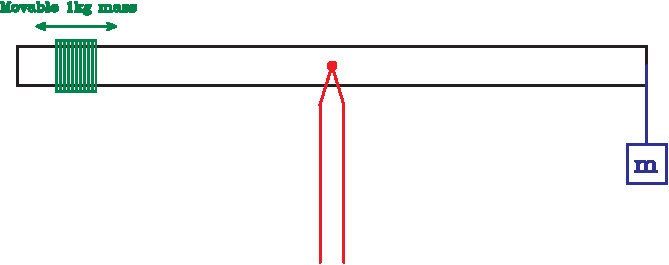
\includegraphics[width=3.5in]{balance-scale-crop.pdf}
\end{center}
\end{minipage}
\bigskip



To measure an unknown mass, you tie the unknown mass to the string at the right side, then slide the mass on the left back and forth until the meter stick is balanced and does not tip one way or the other. \textit{(This happens when the net torque on it is zero.)}



a) Draw an extended force diagram for the meter stick. \textit{(This means you should draw not just a dot, but the entire object. Then label each force at the position where it acts.)}

{\color{red} Here they should have the weight of the known mass (which they will need to label -- perhaps $M$ for its mass, so $Mg$) at its position going downward, $mg$ going downward on the rightmost edge, a normal force/support force going upward at the center, and -- if they think of it -- the weight of the meter stick itself at the center. If they forget about it, they'll discover it later :)}
 
\vspace{3in}

b) In analyzing the torques on this system, you'll need to choose a pivot. It is a good idea to choose the pivot at the location of forces that you {\bf do not know} and {\bf do not care about}. What location should you choose? Label this position on your force diagram.

{\color{red}  The only sensible choice for the pivot is at the location of the support force: we don't know the normal force nor do we care. (We also don't know the weight of the meter stick...) }

\vspace{1in}

\newpage

c) Suppose the system is balanced when you put the movable mass on the 20 cm mark. What is the unknown mass?

{\color{red} Here we write down the net torque, choosing CCW to be positive and CW to be negative, and set it to zero. If the mass is at the 20 cm mark, we know its distance from the pivot is 30 cm. There are four torques: from the movable mass $M$, from the unknown mass $m$, from the support force $F_N$, and from the weight of the stick $M_s$ (which I use $\tau_s$ for). The last two of these are zero since they act at the location of the pivot we chose.
	
	\begin{align*}
		\sum \tau =& 0 \\
		\tau_M + \tau_m + \tau_s + \tau_N =& 0 \\
		M(30\,{\rm cm}) - m(50\,{\rm cm})  =& 0 \\
\end{align*}
	
		and doing a bit of math gives $m = $ 600 grams.
		

  }

\vspace{2in}

d) Another engineering student comes by and wants to modify the device, since they need to measure masses more than 1kg. They shift the support rod to the 80 cm mark. Draw an extended force diagram for the rod now.


{\color{red} Same diagram as before, but the support force is moved.}

\vspace{2in}

e) Referencing the idea of torque, explain in words why this will let you measure heavier masses than attaching the rod to the 50cm mark. Once your group has an explanation, call one of your instructors over and share your explanation with them.

{\color{red} Canonical answer: ``We still choose the pivot at the location of the support force since we don't know and don't care about it. In order to measure a heavier mass than 1 kg, we need its torque to still be counterbalanced by the torque from the 1 kilogram counterweight. To achieve this, we need to move the counterweight further from the pivot than the unknown mass. We can achieve this by shifting the support point -- now the unknown mass is only 20 cm away, but we can move the counterweight up to 80 cm away. We can thus measure stuff of up to around 4 kg (but see next part).}

\vspace{1.5in}

f) Another engineering student comes by and says ``Wait, you won't get very precise measurements out of this unless you measure the mass of the meter stick, too.'' Why does the mass of the meter stick not matter when the support rod is attached at the 50 cm mark, but does matter when it is attached at the 80 cm mark?

{\color{red} Now, since the weight of the meter stick isn't directed at the pivot, it applies a torque too. Before the weight of the meter stick acted at the pivot so we didn't care.}


\newpage


\centerline{\large Question 2: on static equilibrium}



\begin{minipage}[b]{0.4\textwidth}
  \vspace{-0.8in}

A 4m-long pole of mass 80 kg extends from the side of a building, angled at 60 degrees above the horizontal. One meter from the end of the pole, a sign of mass 50 kg is attached. To support the pole,
a horizontal cable runs from the end of the pole to the building. (See the attached figure.)

\bigskip
\bigskip
\bigskip
\bigskip
\bigskip
\bigskip

\end{minipage}
\begin{minipage}[t]{0.6\textwidth}
  \begin{flushright}
  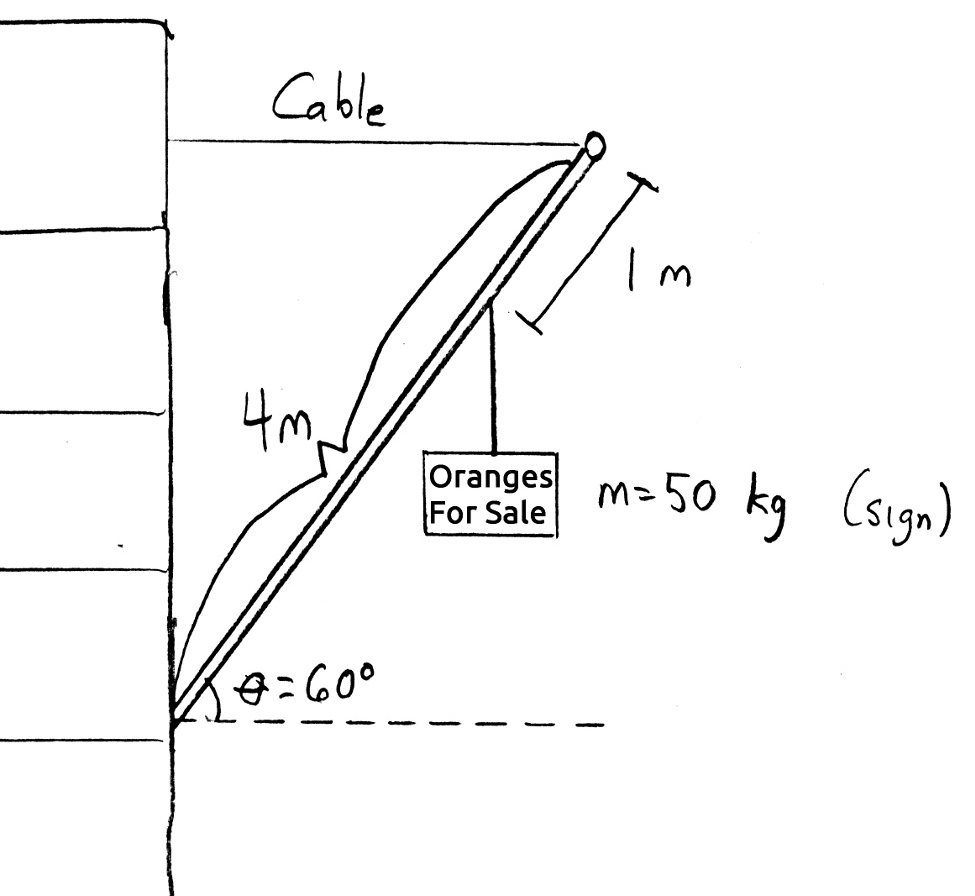
\includegraphics[width=0.9\textwidth]{sign2.jpg}
\end{flushright}
\end{minipage}

\bigskip
\bigskip

\newpage

a) Draw a force diagram, showing all of the elements needed to help you compute the tension in the support cable. Indicate
your choice of pivot point.
{\color{red} 
	
	All the forces go where they go. Note that there is a normal force/attachment force where the pole attaches to the building. We don't know its size or direction, but we should label it. It's a good clue this is where we should choose the pivot to be. Don't forget the weight of the rod (at its center).
}


\newpage

%\begin{landscape}

b) Complete the following table, letting you calculate the torque from every force in the problem. 

{\color{red} Here I label $L$ as the length of the rod and $d$ as 3 meters.}

\large
\begin{center}
\begin{tabular}{|c|c|c|c|c|c|}
\hline
Name & Distance to & Size of force & $\sin \theta$ (angle  & + or - & {\bf Torque} \\
     & pivot ($r$) & (F) & between $\vec F$ and $\vec r$) & & \\\hline
   
     {\color{red} Cable}              &    {\color{red}$L$ (4 m)}                       &  {\color{red}$T$}                       &  {\color{red}$\sin 60^\circ$}                                             &     {\color{red}+}                &      {\color{red}$TL \sin 60^\circ$   }                       \\ \hline
      {\color{red} Weight of rod}         & {\color{red}$L/2$ (2 m)}                        &  {\color{red}$Mg$}                      &     {\color{red}$\sin 30^\circ$}                                         & {\color{red}-}                   &  {\color{red}$-\frac{MgL}{2} \sin 30^\circ$}                             \\ \hline
      {\color{red}Weight of sign}        &       {\color{red}$d$ (3 m)}                  & {\color{red}$mg$}                       &    {\color{red}$\sin 30^\circ$}                                          &   {\color{red}-}                 & {\color{red}$-mgd \sin 30^\circ$}                              \\ \hline
     {\color{red}Hinge force}         &    {\color{red}Zero}                     &     {\color{red}Don't care}                   &     {\color{red}Don't care}                                         &    {\color{red}N/A}                &    {\color{red}Zero}                           \\ \hline
\end{tabular}
\end{center}
\normalsize
c) Compute the tension in the cable.

{\color{red} Students are not going to want to be methodical and fill out the table above. They need to do it anyway.
	
	Then it is as simple as adding up all the torques and setting them to zero. So:
	
	$$TL \sin 60^\circ - \frac{MgL}{2} \sin 30^\circ -mgd \sin 30^\circ + 0 = 0$$
	
	and solve for $T$.
}

\vspace{3 in}

d) Suppose now that the store owner wanted to attach the cable to a different point on the building in order to minimize its tension. What angle between the
cable and the horizontal would support the pole with the minimum tension?
%\end{landscape} 
{\color{red}The CCW torque from the cable needs to balance the CW torque from the weight of the bar and sign. To get the most torque from a given tension, the cable should be perpendicular to the radius vector (i.e. the bar).
}

\newpage

\centerline{\large Question 3: torque in dynamic equilibrium}

A unicyclist rides at a constant speed of 5 m/s; she and her unicycle have a combined mass of 70 kg. The wheel of her unicycle has a radius of 50 cm. At this speed, air resistance exerts a force of 80 N on her.


1) What is the angular velocity of the wheel?
\vspace{1.2in}

{\color{red}
	
	We know that if something rolls without slipping, 
	
	$$v = \omega r$$
	
	which means 
	
	$$\omega = 10 \frac{\text{rad}}{\text{s}}.$$
}


2) As you know, the force that wheeled vehicles use to propel themselves forward is static friction. What is the size of this force?
\vspace {1.2in}

{\color{red} If she's going at a constant speed, $\sum \vec F = 0$, and so the static friction force must be equal to the retarding force from air drag, so $F_{\rm{trac}} = 80 \rm N$.}

3) What torque must she apply to the wheel to maintain her speed? \textit{(Hint: What is the net torque on the wheel?)}
\vspace{2in}

{\color{red} The wheel has $\alpha = 0$, too, which means $\sum \tau = 0$. This means that the torque from traction must be equal and opposite to the torque she applies to the pedals. The torque from fraction is 
	
	$$\tau_{\rm {trac}} = F_\perp r = Fr = 40\,\rm N\cdot \rm m.$$
}

\newpage

4) Suppose the pedals are attached to a crank with a radius of 25 cm. What force must she apply to the pedals to maintain her speed?
\vspace{3in}

{\color{red} She's got to apply an equal and opposite torque to the pedals. If the crank she's using is only 25 cm long, the force she must apply is 160 N. (This is obviously an oversimplification since it assumes she is always pushing perpendicularly.)}

%5) What power does she apply to the pedals? What power does the air resistance apply?
\newpage

\Large
\centerline{\sc{Recitation Exercises}}
\normalsize
\centerline{\sc{April 22}}


\centerline{\large Question 1: on rotational dynamics}
A flywheel (a large, spinning disc) of mass $m$ and radius $r$ is rotating
at angular velocity $\omega$. The machine operator wishes to bring it to rest using a friction brake. When the brake
is engaged, two brake pads on either side of the disc are pressed against it from either side, two-thirds
of the way from the center to the outer edge; each brake pad
exerts a normal force $F_N$.

If the coefficient of friction between the brake pads and the disc is $\mu_k$, how long does it take the
brake to bring the flywheel to a stop?

{\color{red}

This is a pretty simple example : the path to solve it is straight-ahead, but it involves tying together a lot of different things.

This is a two-step process: first we find the $\alpha$ that results from the torque from friction, then we find the time it takes to stop with that angular acceleration.

We know 

$$\tau = I \alpha$$

Here we know $$I=\frac{1}{2}mr^2$$ and $$\tau = F_\perp r = (2 \mu_k F_N)(2/3 r)$$

Substituting gives

$$\frac{4}{3} \mu_k F_N r = \frac{1}{2}mr^2 \alpha \rightarrow \alpha = \frac{8\mu_k F_N}{3mr}$$

Then they need to use some rotational kinematics that they will learn about Thursday to find the time. This includes 
	
	$$\theta(t) = \theta_0 + \omega_0 t + \frac{1}{2}\alpha t^2$$
	
	and
	
	$$\omega(t) = \omega_0 + \alpha t.$$
	
The second equation is what we want. Set $\omega(t)=0$ and solve for $t$ to get

$$t = \frac{3mr\omega_0}{8\mu_k F_N}.$$

}
	
	
	

\newpage
\centerline{\large Question 2: on linked objects}

A bucket of mass $m$ hangs from a string wound around a pulley
(a solid cylinder) with mass $M$ and radius $r$. When the bucket is
released, it falls, unwinding the string.

\begin{enumerate}

\item Draw force diagrams for the bucket and the pulley. Note that since the pulley rotates, you will need
to draw an extended force diagram for it, drawing the object and labeling where each force acts.


{\color{red}
Force diagram for pulley: tension points straight downward from the outside. Optionally: a support force from the axle points straight up, the pulley's own weight points down. These don't matter since the pulley will only rotate, not translate, and thus forces acting at the axle are irrelevant since they apply no torque. Force diagram for bucket: tension points up, gravity points down.}

\vspace{3in}

\item In terms of the forces in your force diagrams, write an expression for the net torque on the pulley.


{\color{red}
Here the only force applying a torque is the rope, so

$$\tau = \pm Tr.$$

Note that this will be either positive or negative depending on which side they've drawn the string on. THIS IS IMPORTANT -- they need to be consistent with their coordinate system.

}
\vspace{1in}

\item Write down Newton's laws of motion -- $\sum \vec F = m \vec a$ for translation, and $\sum \tau = I \alpha$
-- for each object. (One object moves, and the other turns...)


{\color{red}
For the bucket:

$$T - mg = ma$$

For the pulley, for instance (using a coordinate system where CCW is positive and the rope pulls on the right):

$$\tau = I \alpha \rightarrow -Tr = I \alpha \rightarrow -Tr = \frac{1}{2}Mr^2 \alpha$$


}

\vspace{2in}


\newpage

\item What is the relationship between the angular acceleration $\alpha$ of the pulley and the linear acceleration
$a$ of the bucket? (The answer may be different depending on how you have drawn your pictures and your choice of
coordinate system.)


{\color{red}

For my choice, the spool rotates CW (negative) while the bucket falls down (negative). So $a = \alpha r$. {\bf Depending on their choices}, it may be the other way around. There will be a negative sign either here or in the value of torque.

}

\vspace{1in}

\item Calculate the acceleration of the bucket in terms of $m$ and $M$.


{\color{red}

System of two equations. First we fix up the rotation equation a little bit:

$$-Tr = \frac{1}{2}Mr^2 \alpha \rightarrow -T = \frac{1}{2}Mr\alpha \rightarrow T = -\frac{1}{2}Ma$$

where we've cancelled an $r$ and then substituted the constraint $a = \alpha r$ in.

Then we substitute this into the translation equation:

$$-\frac{1}{2}Ma - mg = ma  \rightarrow a = \frac{-mg}{m+\frac{1}{2}M}$$





}


\vspace{3in}

\item Suppose that the pulley were a hollow cylinder with the same mass. How would this acceleration change?

 
 {\color{red}
This only changes $I$. Here the cylindrical nature was encoded in the factor of 1/2 in $I$. Repeating the above generically for $I=\lambda mr^2$ and following everything through gives


 $$a = \frac{-mg}{m+\lambda M}$$
 
 and putting in $\lambda=1$ (hollow cylinder) gives
 
 $$a = \frac{-mg}{m+M}$$
}
 


\end{enumerate}
\end{document}
